\chapter{Prestudent}
\label{prestudent}
\section{Aufbau der Karteikarte Prestudent}
\begin{figure}
	\centering
	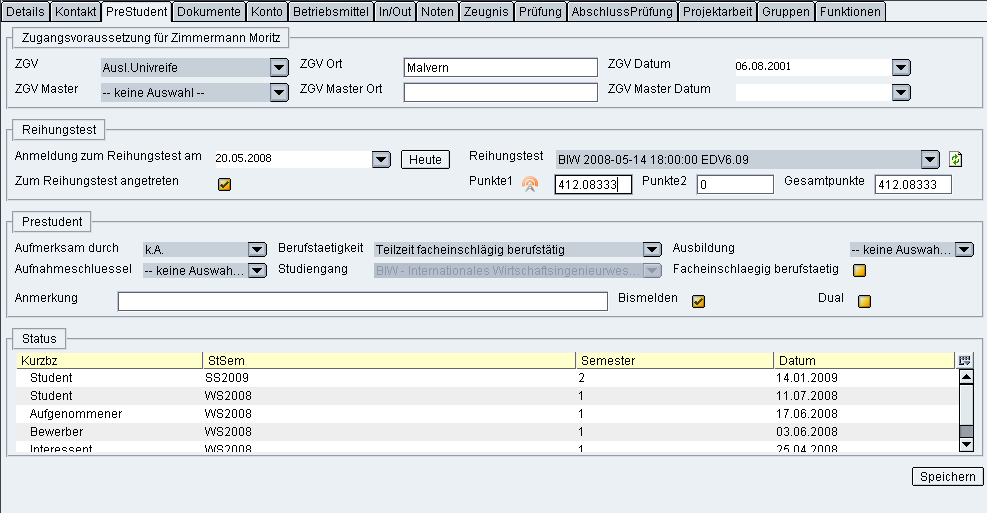
\includegraphics[width=0.75\textwidth]{FAS_Prestudent1.png}
	\caption{Die Karteikarte Prestudent}
	\label{Prestudent1}
\end{figure}
\begin{itemize}
	\item Zugangsvoraussetzungen: 	
	\begin{itemize}
		\item ZGV: Zugangsvoraussetzungen, die zu einer Teilnahme an einem Diplom- oder Bachelorstudiengang berechtigt. Schultyp und Datum des Abschlu�zeugnisses sind Teil der Studenten-BIS-Meldung.
		\item ZGV Master: Zugangsvoraussetzung, die zu einer Reilnahme an einem Masterstudiengang berechtigen.
	\end{itemize}
\achtung{\textbf{Wichtig} Die BIS-Meldung verlangt in Masterstudieng�ngen die Eintragung beider Zugangsvorraussetzungen!}\\

\idee{\textbf{Tipp} Bei Interessenten, die ihren Abschlu� noch nicht gemacht haben, sollte f�r die Interessentenstatistik die ZGV m�glichst fr�h bereits eingegeben werden! Das ZGV-Datum wird dann nach der bestandenen Pr�fung eingetragen.}\\

	\item Reihungstest: 
	\begin{itemize}
		\item Anmeldung zum Reihungstest am: Hier kann das Datum der Anmeldung zum Reihungstest eingegeben oder mit dem Kalendertool ausgew�hlt werden. Die rechts vom Eingabefeld befindliche Taste \textit{Heute} setzt das aktuelle Datum in das Eingabefeld. Bei der Inskription mu� das Datum eingegeben sein.
		\item Reihungstest: Auswahl des Reihungstests. Beim Speichern wird gepr�ft, ob diese Person in einem anderen Studiengang des selben Typs (Master, Bachelor,...) bereits einen Reihungstesttermin hat. Falls dies der Fall ist, wird eine Warnung angezeigt. Die Daten trotzdem gespeichert.
		Rechts neben dem Auswahlfeld befindet sich 
\includegraphics{icon_aktualisieren}, eine Aktualisierungstaste. Dieser kann verwendet werden, um die Liste zu aktualisieren, wenn ein neuer Reihungstesttermin �ber die Reihungstestverwaltung angelegt wird.
		\item Zum Reihungstest angetreten: Zeigt an, ob der Bewerber zu einem Reihungstest angetreten ist. Bei aktiven Studenten mu� das H�kchen gesetzt sein (BIS-Meldung).
		\item Reihungstestpunkte: Die Reihungstestpunkte sind in 3 Felder unterteilt. Das Feld Punkte1 sind die Punkte des elektronischen Reihungstests. Die Punkte des Testtools k�nnen automatisch �bernommen werden wenn auf das Symbol neben dem Eingabefeld geklickt wird. (Die Punkte aus dem Dynamic Power Trainer k�nnen hier nicht automatisch �bernommen werden.) Das Feld Punkte2 enth�lt die Punkte des Pers�nlichen Gespr�chs bzw weitere Aufnahmekriterien (Sporttest). Das 3. Feld enth�lt die Gesamtpunkte. Diese werden in der Regel automatisch aus den beiden anderen Feldern berechnet. 
	\end{itemize}
	\item Prestudent:
	\begin{itemize}
		\item Aufmerksam durch: Auswahl, wodurch der Student auf den Studiengang aufmerksam wurde. 
		\item Berufstaetigkeit: 
		\item Ausbildung: Eingabe der h�chsten abgeschlossenen Ausbildung.
		\item Aufnahmeschluessel
		\item Studiengang: Zeigt den Studiengang an.
		\item Facheinschlaegig berufstaetig: 
		\item Anmerkung: Hier k�nnen zus�tzliche Informationen eingegeben werden.
		\item Bismelden: Bestimmt, ob Student in die BIS-Meldung gelangt. Das H�kchen ist standardm��ig gesetzt.\\
		\underline{Beispiel}:\\
		Student XY inskribiert im Juni das n�chste Wintersemester im Studiengang YZ. Am 17.Oktober gibt der Student aber das Studium auf. Vorgehensweise: Der Status des Studenten wird auf \textsl{Abbrecher} gesetzt. Danach wird das \textsl{Aktiv}-H�kchen in der Karteikarte \textit{Details} und das \textsl{Bismelden}-H�kchen entfernt. Somit wird der Student zum Abbrecher gemacht und nicht in der n�chsten BIS-Meldung am 15.November gemeldet.\\
	\end{itemize} 
	\item Status: Dieser Bereich besteht aus einer Liste aller Stati des ausgew�hlten Studenten.
\end{itemize}
\achtung{\textbf{Wichtig} Bei der BIS-Meldung d�rfen keine Studienanf�nger gemeldet werden, die vor dem Stichtag der ersten BIS-Meldung das Studium abgebrochen haben!}\\

\section{Rechtsklick-Funktionen}
Im Listenfeld \textit{Status} gibt es drei Funktionen, die mit einem Rechtsklick aufgerufen werden:
\begin{itemize}
	\item Bearbeiten: Bei einem im Listenfeld markierten Status k�nnen folgende Daten ver�ndert werden:
	\begin{itemize}
		\item Studiensemester
		\item Ausbildungssemester
		\item Datum
	\end{itemize}
	\item Neuen Status einfuegen: Hier kann dem Studenten ein neuer Status hinzugef�gt werden. \\
	Einschr�nkungen:	
	\begin{itemize}
		\item Es k�nnen nur die Stati \textit{Interessent}, \textit{Bewerber} und \textit{Student} gesetzt werden.
		\item Der Status \textit{Student} kann nur eingef�gt werden, wenn der Student bereits einen Status \textit{Student} besitzt, also schon inskribiert ist. Die Inskription erfolgt mittels \textit{Status �ndern}, wie im Kapitel \ref{ManuellerStatus} beschrieben.
		\item Es k�nnen keine zwei gleiche Stati im selben Studiensemester eingegeben werden.
	\end{itemize}
	\item Entfernen: Hier kann ein markierter Status gel�scht werden.\\
	Einschr�nkungen:
	\begin{itemize}
		\item Es k�nnen alle bis auf einen Status gel�scht werden.
		\item Studentenstati k�nnen nur vom Administrator entfernt werden.
	\end{itemize}
\end{itemize}
\newpage
\label{pflichtpre}
\section{Pflichtfelder}
\begin{figure}
	\centering
	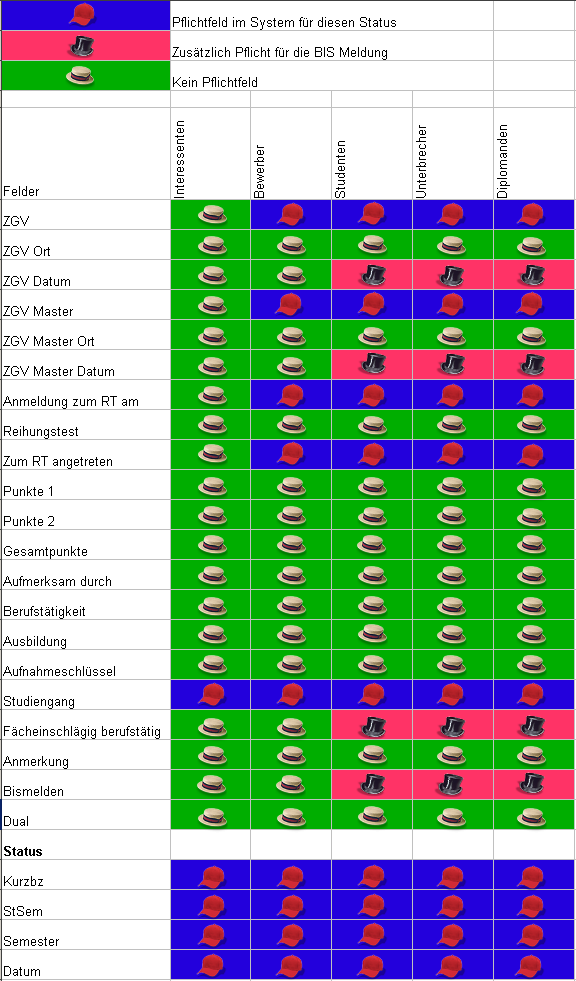
\includegraphics[width=0.70\textwidth]{FAS_Pflichtfelder_PreStudent.png}
	\caption{Die Pflichtfelder des Karteireiters Prestudent}
	\label{Bild_Pflichtpre}
\end{figure}